\documentclass[a4paper]{article}
\usepackage{german}
\usepackage[utf8]{inputenc}

\usepackage{pgfplots}
\usepackage{pgfplots.assert}

\usepgfplotslibrary{fillbetween}

\begin{document}

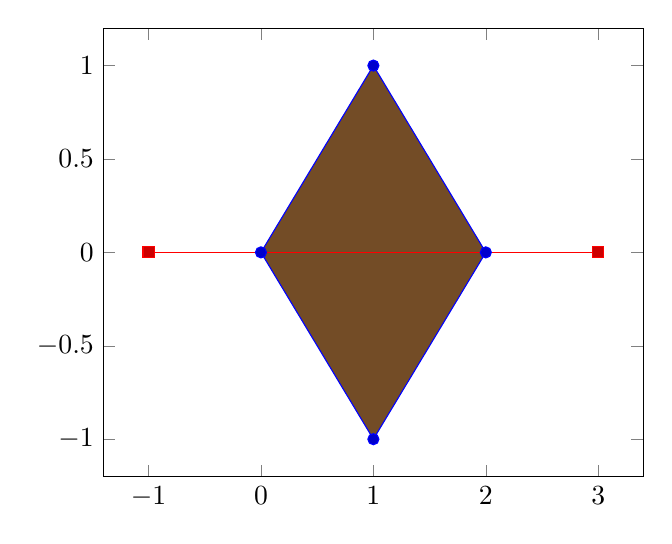
\begin{tikzpicture}
%\tracingcommands=2\tracingmacros=2
\begin{axis}
	\addplot+[name path=A] coordinates {
		  (0,0) (1,1) (2,0) (1,-1)
	} --cycle;

	\addplot+[name path=B]  coordinates {
		(-1,0) (3,0)
	};

	\addplot fill between[of=A and B];

\end{axis}
\end{tikzpicture}

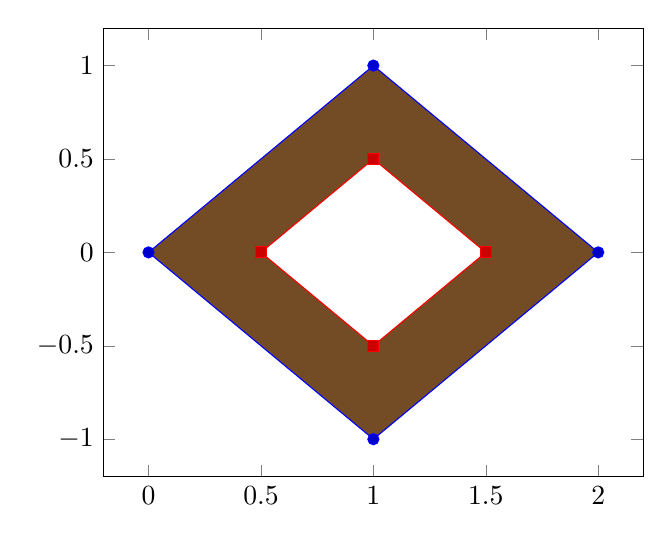
\begin{tikzpicture}
%\tracingcommands=2\tracingmacros=2
\begin{axis}
	\addplot+[name path=A] coordinates {
		  (0,0) (1,1) (2,0) (1,-1)
	} --cycle;

	\addplot+[name path=B]  coordinates {
		  (0.5,0) (1,0.5) (1.5,0) (1,-0.5)
	} -- cycle;

	\addplot+[even odd rule] fill between[of=A and B];

\end{axis}
\end{tikzpicture}

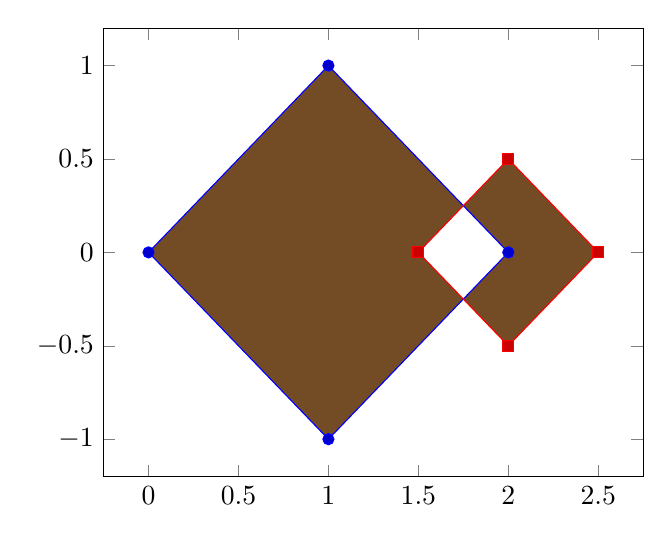
\begin{tikzpicture}
%\tracingcommands=2\tracingmacros=2
\begin{axis}
	\addplot+[name path=A] coordinates {
		  (0,0) (1,1) (2,0) (1,-1)
	} --cycle;

	\addplot+[name path=B]  coordinates {
		  (1.5,0) (2,0.5) (2.5,0) (2,-0.5)
	} -- cycle;

	\addplot+[even odd rule] fill between[of=A and B];

\end{axis}
\end{tikzpicture}

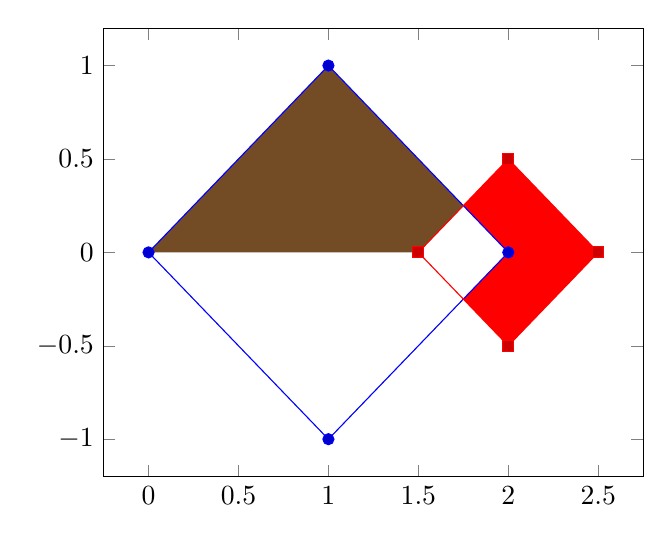
\begin{tikzpicture}
%\tracingcommands=2\tracingmacros=2
\begin{axis}
	\addplot+[name path=A] coordinates {
		  (0,0) (1,1) (2,0) (1,-1)
	} --cycle;

	\addplot+[name path=B]  coordinates {
		  (1.5,0) (2,0.5) (2.5,0) (2,-0.5)
	} -- cycle;

	\addplot+[even odd rule] fill between[of=A and B,
		split,
		every segment no 1/.style={red}];

\end{axis}
\end{tikzpicture}
\end{document}

